% Chapter Template

\chapter{Cross-Encoder Architecture and Training Framework} % Main chapter title

\label{Chapter4} % Change X to a consecutive number; for referencing this chapter elsewhere, use \ref{Chapter4}

%----------------------------------------------------------------------------------------

\section{Cross-Encoder Architecture for Information Retrieval}

\subsection{Architectural Overview}

Cross-encoder models represent a significant advancement in neural information retrieval, enabling deep interaction modeling between queries and documents. Unlike bi-encoder approaches that process queries and documents independently, cross-encoders perform joint encoding, allowing for rich token-level interactions that lead to superior relevance estimation.

\begin{figure}[H]
    \centering
    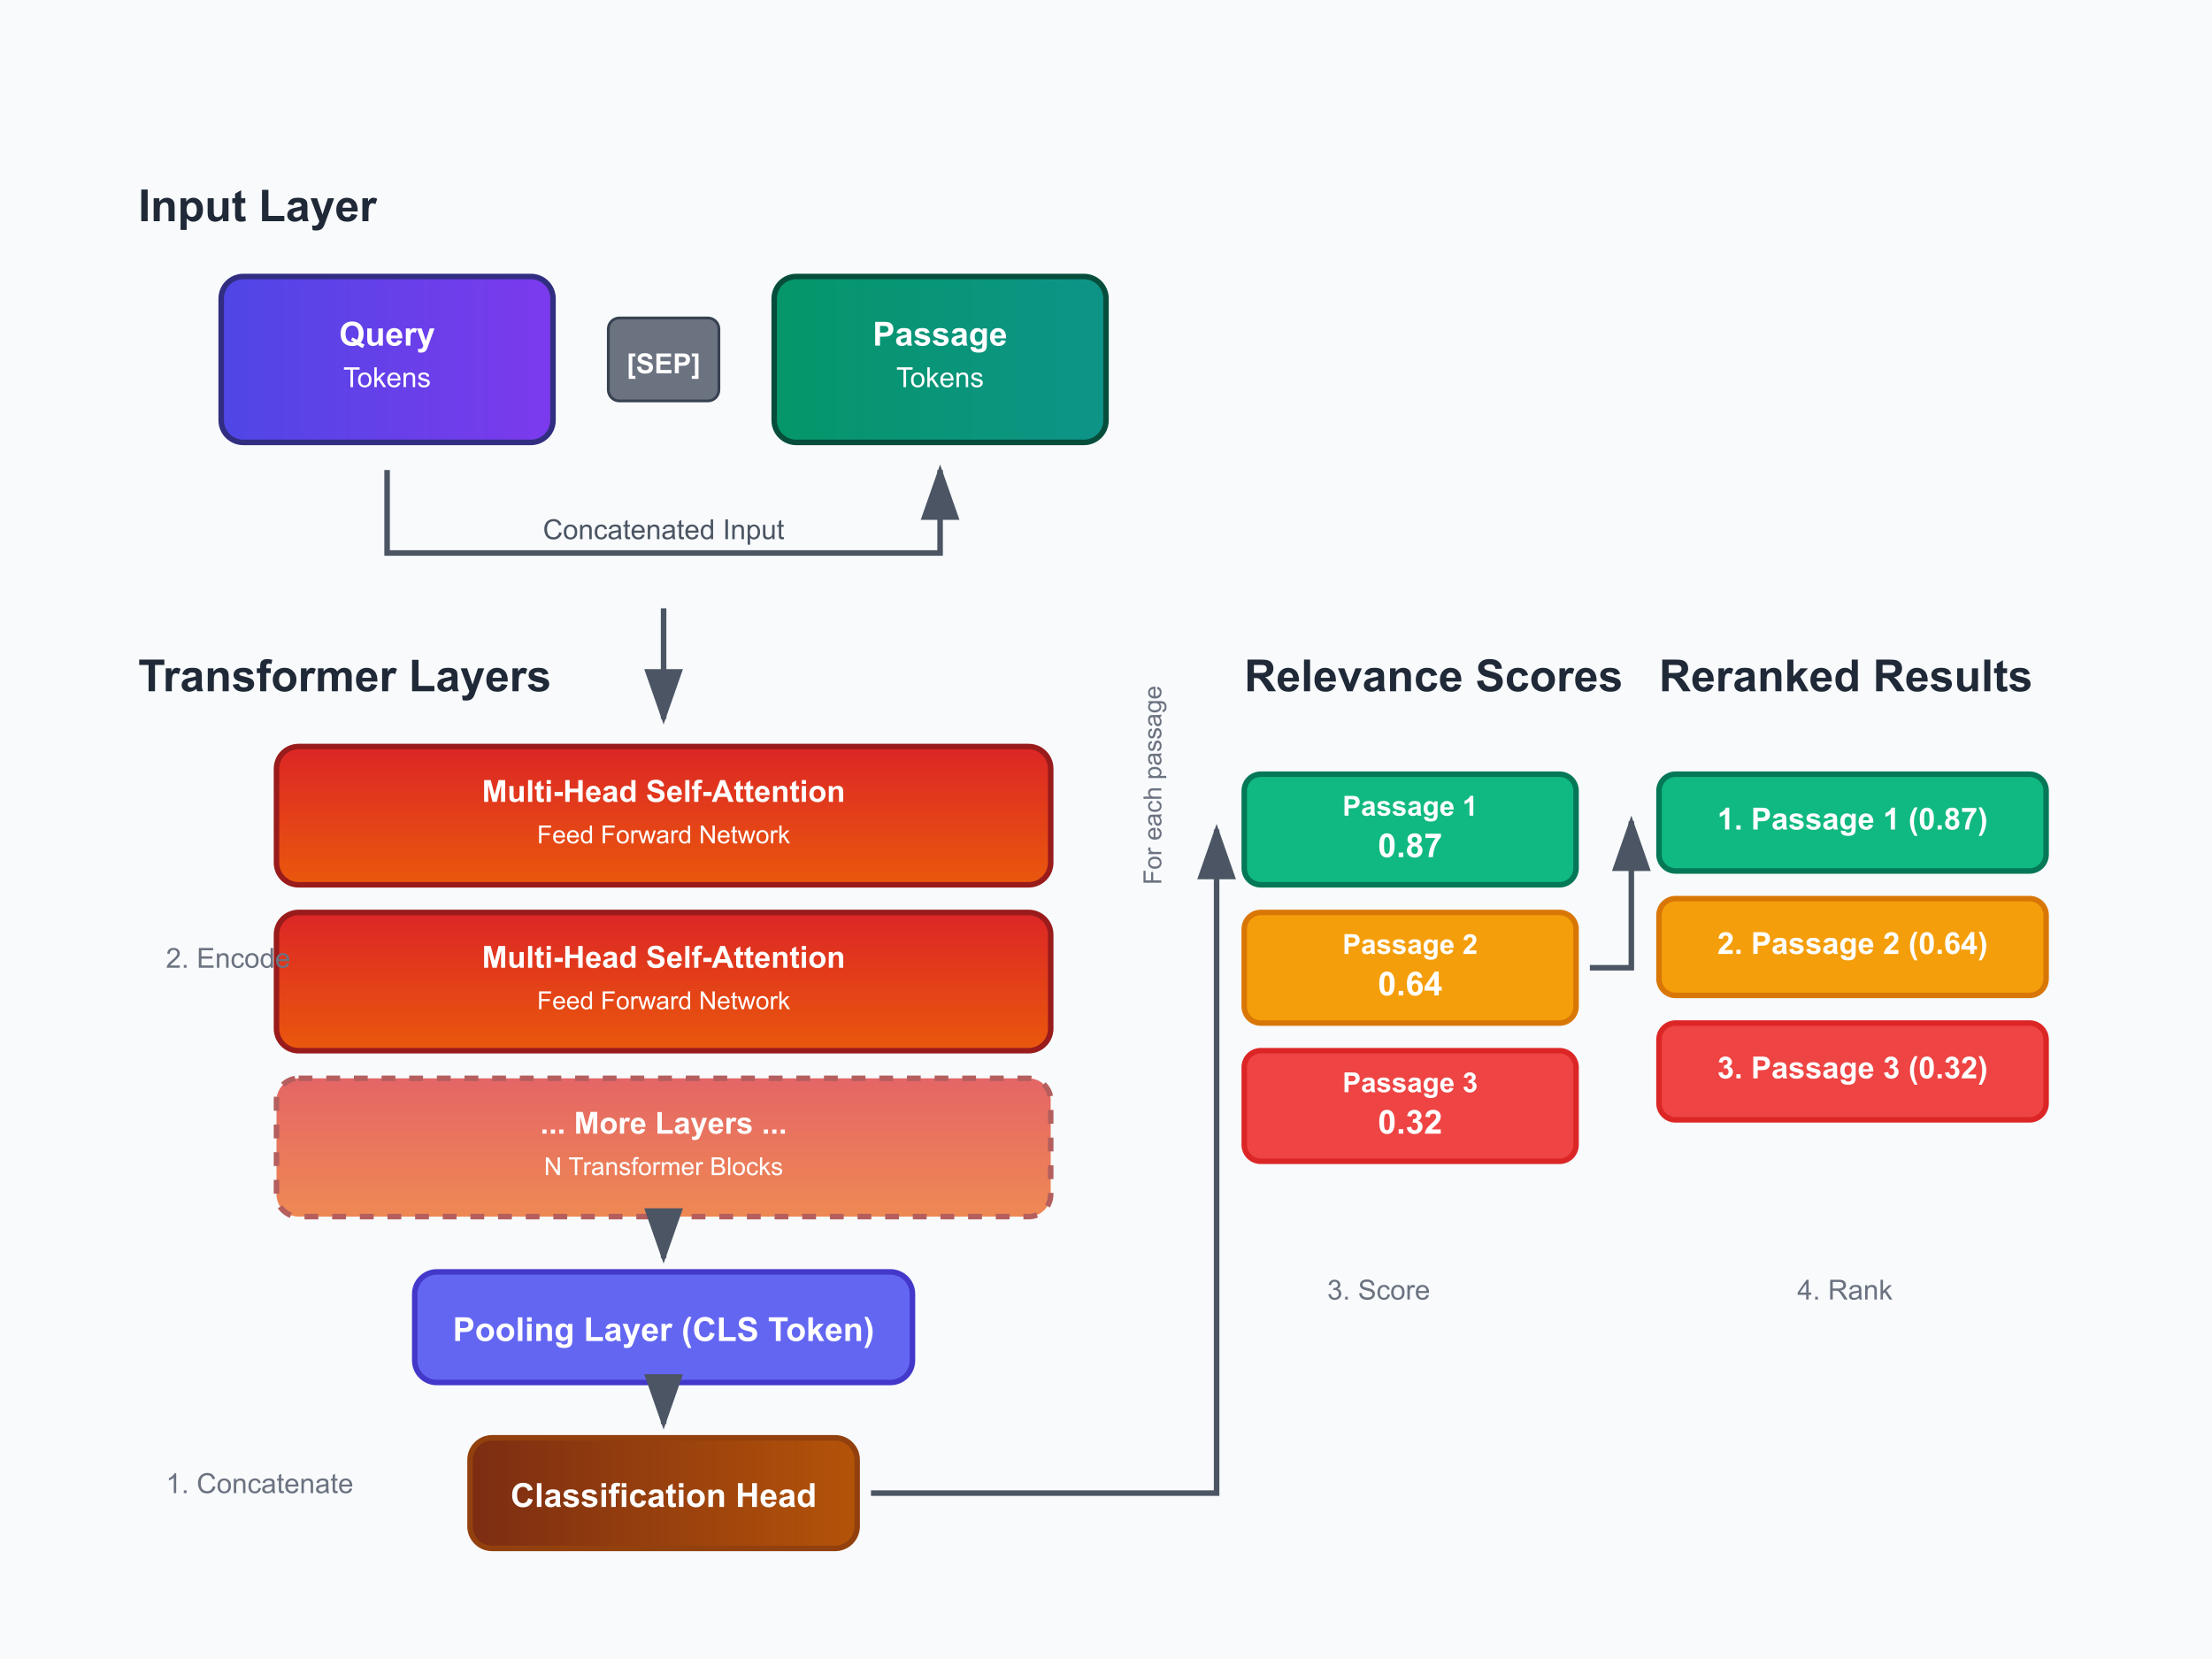
\includegraphics[width=\textwidth]{Figures/cross_encoder_diagram.png}
    \captionsetup{font=footnotesize, width=0.9\linewidth}
    \caption{Cross-Encoder Architecture for Passage Reranking. The model processes concatenated query-passage pairs through transformer layers, producing relevance scores for reranking candidate documents.}
    \label{fig:cross_encoder_architecture}
\end{figure}

The cross-encoder architecture follows a structured approach to relevance modeling:

\begin{enumerate}
    \item \textbf{Input Formatting}: Query and passage text are concatenated with special tokens: [CLS] query [SEP] passage [SEP]
    \item \textbf{Tokenization}: The input sequence is tokenized using subword tokenization (typically BERT-style WordPiece)
    \item \textbf{Transformer Encoding}: The concatenated sequence passes through multiple transformer layers with self-attention mechanisms
    \item \textbf{Relevance Prediction}: The [CLS] token representation is fed to a classification head producing a relevance score
    \item \textbf{Score Normalization}: Sigmoid activation ensures scores fall within [0,1] range for ranking
\end{enumerate}

\subsection{Model Architecture Specifications}

Three distinct transformer architectures were selected to represent different efficiency-effectiveness trade-offs:

\subsubsection{MiniLM-L12-H384-uncased}

MiniLM \cite{wang2020minilm} represents an efficient architecture designed through knowledge distillation:

\textbf{Architectural Parameters}:
\begin{itemize}
    \item Hidden dimensions: 384
    \item Number of layers: 12
    \item Attention heads: 12
    \item Maximum sequence length: 512 tokens
    \item Parameter count: ~33M parameters
    \item Vocabulary size: 30,522 tokens
\end{itemize}

\textbf{Design Philosophy}: MiniLM achieves efficiency through knowledge distillation from larger teacher models while maintaining competitive performance. The reduced hidden dimensions and moderate layer count make it suitable for resource-constrained scenarios while preserving essential language understanding capabilities.

\subsubsection{GTE-multilingual-base}

The General Text Embeddings (GTE) model \cite{li2023towards} extends capabilities to multilingual contexts with enhanced capacity:

\textbf{Architectural Parameters}:
\begin{itemize}
    \item Hidden dimensions: 768
    \item Number of layers: 12
    \item Attention heads: 12
    \item Maximum sequence length: 8192 tokens
    \item Parameter count: ~305M parameters
    \item Vocabulary size: 250,048 tokens
    \item Multilingual vocabulary support
\end{itemize}

\textbf{Design Philosophy}: GTE models are trained on diverse, multilingual corpora with multi-stage contrastive learning. The extended context length (8192 tokens) enables processing of longer documents, making it particularly suitable for comprehensive passage analysis and cross-lingual retrieval scenarios.

\subsubsection{ModernBERT-base}

ModernBERT \cite{modernbert} incorporates state-of-the-art architectural innovations for improved efficiency and effectiveness:

\textbf{Architectural Parameters}:
\begin{itemize}
    \item Hidden dimensions: 768
    \item Number of layers: 22
    \item Attention heads: 12
    \item Maximum sequence length: 8192 tokens
    \item Parameter count: ~149M parameters
    \item Vocabulary size: 50,368 tokens
    \item Advanced positional encoding and attention mechanisms
\end{itemize}

\textbf{Architectural Innovations}:
\begin{enumerate}
    \item \textbf{Rotary Position Embedding (RoPE)} \cite{su2023roformerenhancedtransformerrotary}: Enables effective handling of longer sequences through relative position encoding
    \item \textbf{Flash Attention} \cite{dao2022flashattentionfastmemoryefficientexact}: Improves memory efficiency and computational speed for attention operations
    \item \textbf{GeGLU Activation Functions} \cite{shazeer2020gluvariantsimprovetransformer}: Enhances model expressiveness while maintaining computational efficiency
\end{enumerate}

\textbf{Design Philosophy}: ModernBERT represents the current state-of-the-art in encoder-only transformers, combining architectural efficiency improvements with enhanced sequence processing capabilities. The deeper architecture (22 layers) with efficient attention mechanisms enables superior language understanding while maintaining practical computational requirements.

%----------------------------------------------------------------------------------------

\section{Optimizer Analysis and Implementation}

\subsection{AdamW Optimizer}

AdamW \cite{loshchilov2019decoupled} has established itself as the standard optimizer for transformer-based models through improved handling of weight decay regularization.

\subsubsection{Mathematical Formulation}

The AdamW update rule decouples weight decay from gradient-based updates:

\begin{align}
m_t &= \beta_1 m_{t-1} + (1 - \beta_1) g_t \\
v_t &= \beta_2 v_{t-1} + (1 - \beta_2) g_t^2 \\
\hat{m}_t &= \frac{m_t}{1 - \beta_1^t} \\
\hat{v}_t &= \frac{v_t}{1 - \beta_2^t} \\
\theta_t &= \theta_{t-1} - \eta \left( \frac{\hat{m}_t}{\sqrt{\hat{v}_t} + \epsilon} + \lambda \theta_{t-1} \right)
\end{align}

where:
\begin{itemize}
    \item $g_t$: gradient at time step $t$
    \item $m_t$: exponential moving average of gradients (momentum)
    \item $v_t$: exponential moving average of squared gradients
    \item $\eta$: learning rate
    \item $\lambda$: weight decay coefficient
    \item $\beta_1, \beta_2$: exponential decay rates for moment estimates
\end{itemize}

\subsubsection{Key Advantages}

\begin{enumerate}
    \item \textbf{Decoupled Weight Decay}: Separates regularization from adaptive learning rate scaling
    \item \textbf{Adaptive Learning Rates}: Per-parameter learning rate adaptation based on gradient history
    \item \textbf{Momentum Integration}: Incorporates momentum for improved convergence in consistent directions
    \item \textbf{Robustness}: Proven effectiveness across diverse transformer architectures and tasks
\end{enumerate}

\subsection{Lion Optimizer}

The Lion (Evolved Sign Momentum) optimizer \cite{chen2023symbolic} represents a novel approach discovered through symbolic mathematics and program search.

\subsubsection{Mathematical Formulation}

Lion utilizes a simplified update mechanism based on momentum and sign operations:

\begin{align}
c_t &= \beta_1 m_{t-1} + (1 - \beta_1) g_t \\
\theta_t &= \theta_{t-1} - \eta \left( \text{sign}(c_t) + \lambda \theta_{t-1} \right) \\
m_t &= \beta_2 m_{t-1} + (1 - \beta_2) g_t
\end{align}

where:
\begin{itemize}
    \item $c_t$: interpolated momentum for update direction
    \item $\text{sign}(\cdot)$: element-wise sign function
    \item Other parameters follow similar definitions as AdamW
\end{itemize}

\subsubsection{Key Innovations}

\begin{enumerate}
    \item \textbf{Sign-based Updates}: Uses only gradient direction, not magnitude, for parameter updates
    \item \textbf{Memory Efficiency}: Maintains only first-moment estimates, reducing memory requirements by ~50\%
    \item \textbf{Computational Simplicity}: Sign operation is computationally cheaper than square root calculations
    \item \textbf{Robust Performance}: Demonstrated effectiveness across computer vision and vision-language tasks
\end{enumerate}

\subsubsection{Theoretical Advantages}

The sign-based update mechanism provides several theoretical benefits:

\begin{itemize}
    \item \textbf{Noise Resistance}: Sign operation filters out gradient noise while preserving direction information
    \item \textbf{Scale Invariance}: Updates are independent of gradient magnitude, providing consistent step sizes
    \item \textbf{Convergence Properties}: Simplified dynamics may lead to more stable convergence in some scenarios
\end{itemize}

%----------------------------------------------------------------------------------------

\section{Training Framework and Implementation}

\subsection{Data Preprocessing and Input Formatting}

\subsubsection{Dataset Preparation}

The MS MARCO Passage Ranking dataset \cite{DBLP:journals/corr/NguyenRSGTMD16} serves as the primary training corpus:

\begin{itemize}
    \item \textbf{Training Queries}: 502,939 queries with relevance labels
    \item \textbf{Passage Collection}: 8.8M unique passages
    \item \textbf{Relevance Judgments}: Binary labels indicating passage relevance to queries
    \item \textbf{Data Source}: Real user queries from Bing search engine with human-annotated relevance
\end{itemize}

\subsubsection{Input Processing Pipeline}

\textbf{Text Preprocessing}:
\begin{enumerate}
    \item Unicode normalization and cleaning
    \item Whitespace normalization
    \item Special character handling for robustness
\end{enumerate}

\textbf{Sequence Construction}:
\begin{enumerate}
    \item Query-passage concatenation: [CLS] query [SEP] passage [SEP]
    \item Tokenization using model-specific tokenizers
    \item Sequence length truncation based on model capacity
    \item Attention mask creation for proper sequence processing
\end{enumerate}

\textbf{Batch Construction}:
\begin{enumerate}
    \item Dynamic padding to maximum sequence length in batch
    \item Label tensor creation for binary classification
    \item Efficient DataLoader implementation with multi-processing
\end{enumerate}

\subsection{Training Configuration}

\subsubsection{Hyperparameter Settings}

\textbf{Model-Specific Configurations}:

\begin{table}[h!]
\centering
\begin{tabular}{|l|c|c|c|}
\hline
\textbf{Parameter} & \textbf{MiniLM} & \textbf{GTE} & \textbf{ModernBERT} \\
\hline
Learning Rate & 2e-5 & 2e-5 & 2e-6 \\
\hline
Max Sequence Length & 512 & 8192 & 8192 \\
\hline
Batch Size & 16 & 16 & 16 \\
\hline
Weight Decay & 0.01 & 0.01 & 0.01 \\
\hline
Warmup Steps & 1000 & 1000 & 1000 \\
\hline
LR Scheduler & None & None & Cosine Annealing \\
\hline
Training Epochs & 3 & 3 & 3 \\
\hline
\end{tabular}
\caption{Model-specific training configurations for optimal performance}
\label{tab:training_config}
\end{table}

\textbf{Optimizer-Specific Parameters}:

\begin{table}[h!]
\centering
\begin{tabular}{|l|c|c|}
\hline
\textbf{Parameter} & \textbf{AdamW} & \textbf{Lion} \\
\hline
$\beta_1$ & 0.9 & 0.9 \\
\hline
$\beta_2$ & 0.999 & 0.99 \\
\hline
$\epsilon$ & 1e-8 & - \\
\hline
Gradient Clipping & 1.0 & 1.0 \\
\hline
\end{tabular}
\caption{Optimizer-specific parameter configurations}
\label{tab:optimizer_config}
\end{table}

\subsubsection{Training Objectives}

\textbf{Loss Function}: Binary Cross-Entropy Loss for relevance prediction:

\begin{equation}
\mathcal{L}_{BCE} = -\frac{1}{N} \sum_{i=1}^{N} [y_i \log(\hat{y}_i) + (1-y_i) \log(1-\hat{y}_i)]
\end{equation}

where $y_i$ represents the true relevance label and $\hat{y}_i$ is the predicted relevance score.

\textbf{Regularization Strategies}:
\begin{itemize}
    \item Weight decay regularization (L2 penalty)
    \item Gradient clipping for training stability
    \item Early stopping based on validation performance
\end{itemize}

\subsection{Infrastructure and Implementation}

\subsubsection{Computational Resources}

\textbf{Hardware Platform}: Modal cloud computing platform \cite{modal_labs}
\begin{itemize}
    \item GPU: NVIDIA A100-80GB
    \item Memory: High-bandwidth memory for large model training
    \item Storage: Fast SSD storage for efficient data loading
    \item Network: High-speed interconnects for distributed training
\end{itemize}

\textbf{Software Stack}:
\begin{itemize}
    \item Framework: PyTorch \cite{paszke2019pytorchimperativestylehighperformance}
    \item Model Library: Sentence Transformers \cite{reimers2019sentence}
    \item Evaluation Tools: TREC Eval \cite{trec_eval_github}, Pyserini \cite{lin2021pyserini}
    \item Experiment Tracking: Weights \& Biases \cite{wandb2020}
\end{itemize}

\subsubsection{Training Pipeline}

\textbf{Model Initialization}:
\begin{enumerate}
    \item Load pre-trained transformer weights
    \item Initialize classification head for relevance prediction
    \item Set up optimizer with appropriate hyperparameters
    \item Configure learning rate scheduler if applicable
\end{enumerate}

\textbf{Training Loop}:
\begin{enumerate}
    \item Forward pass through cross-encoder model
    \item Compute binary cross-entropy loss
    \item Backward propagation with gradient computation
    \item Optimizer step with gradient clipping
    \item Learning rate scheduling update
    \item Validation evaluation at specified intervals
\end{enumerate}

\textbf{Model Checkpointing}:
\begin{itemize}
    \item Save model state at each epoch
    \item Track best model based on validation metrics
    \item Enable training resumption from checkpoints
    \item Model versioning for reproducibility
\end{itemize}

This comprehensive training framework ensures consistent and reproducible comparison between Lion and AdamW optimizers across different model architectures while maintaining state-of-the-art training practices for cross-encoder models in information retrieval.


\section{Implementation Considerations}

\subsection{Computational Resources}
The experimental setup requires significant computational resources due to the intensive nature of cross-encoder training. Modal cloud platform provides the necessary GPU resources with NVIDIA A100 instances, ensuring consistent hardware configuration across all experiments.

Resource allocation considerations include:
\begin{itemize}
    \item GPU memory requirements varying by model size (8GB for MiniLM, 16GB for GTE, 24GB for ModernBERT)
    \item Batch size optimization based on available memory
    \item Distributed training capabilities for larger models
    \item Checkpoint storage and management
\end{itemize}

\subsection{Reproducibility Framework}
Ensuring reproducible results across different runs and environments requires careful attention to:

\textbf{Random Seed Management}:
\begin{itemize}
    \item Fixed seeds for PyTorch, NumPy, and Python random modules
    \item Deterministic CUDA operations where possible
    \item Consistent data shuffling across experiments
\end{itemize}

\textbf{Environment Specification}:
\begin{itemize}
    \item Docker containerization for consistent software environments
    \item Dependency version pinning in requirements files
    \item Hardware specification documentation
    \item Environment variable standardization
\end{itemize}

\subsection{Evaluation Pipeline}
The evaluation pipeline ensures consistent and fair comparison between optimizers:

\textbf{Model Loading and Inference}:
\begin{itemize}
    \item Standardized model loading procedures
    \item Consistent tokenization and preprocessing
    \item Batch size optimization for inference efficiency
    \item GPU memory management during evaluation
\end{itemize}

\textbf{Metric Computation}:
\begin{itemize}
    \item Implementation of standard IR metrics (nDCG, MAP, MRR)
    \item Statistical significance testing procedures
    \item Result aggregation and reporting mechanisms
    \item Cross-validation protocols for robust evaluation
\end{itemize}

\section{Chapter Summary}

This chapter presented a comprehensive methodology for comparing Lion and AdamW optimizers in cross-encoder architectures for information retrieval. The systematic approach encompasses model architecture specifications, optimizer implementations, training frameworks, and evaluation protocols.

Key methodological contributions include:

\begin{itemize}
    \item \textbf{Systematic Architecture Comparison}: Detailed specifications for MiniLM, GTE, and ModernBERT cross-encoder implementations, enabling fair comparison across different model scales and designs.
    
    \item \textbf{Rigorous Optimizer Implementation}: Mathematical formulations and computational implementations of both Lion and AdamW optimizers, ensuring consistent comparison conditions.
    
    \item \textbf{Standardized Training Protocol}: Comprehensive training framework with hyperparameter optimization, regularization strategies, and monitoring systems for reproducible results.
    
    \item \textbf{Robust Evaluation Framework}: Multi-dataset evaluation protocol using TREC 2019 and MS MARCO benchmarks with statistical significance testing.
\end{itemize}

The methodology establishes a foundation for systematic optimizer comparison in neural information retrieval, providing insights into the relationship between optimization algorithms and model architectures. The next chapter presents the comprehensive experimental results obtained through this methodological framework.
 

